\section{单图像去雾}
\label{s3}



基于大气模型的SID算法的流程基本上大同小异,我复现以下的几种算法也是一样,一般来说这类SID的流程如图\ref{fig-dehazy}所示,其中边界函数的计算只在一些算法中采用。

\begin{figure}[htbp]
    \centering
    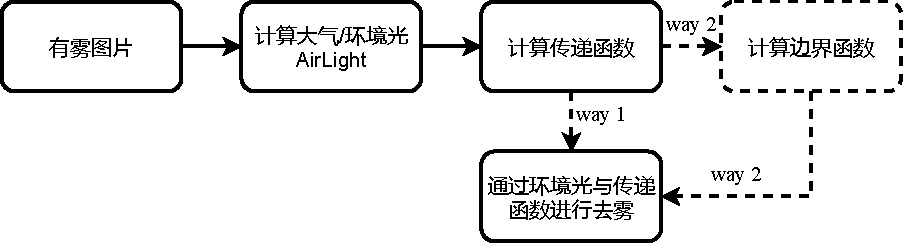
\includegraphics[width=0.8\textwidth]{./imgs/dehazy.pdf}
    \caption{去雾算法流程}
    \label{fig-dehazy}
 \end{figure}

\subsection{基于暗通道先验知识的单图像去雾}
何恺明团队在2009年的CVPR会议中提出暗通道先验(dark channel prior,DCP)算法(后发到TPAMI\cite{he.tang201112})。他们经过大量实验发现,除了亮区或天空区DCP是完全黑暗的,在所有的颜色通道中至少存在一个接近0的亮度值的像素。导致这种现象的原因为:每一张图片中不同物体互相遮挡形成的阴影、图像包括一个颜色接近RGB纯色的区域或者图片的整体风格接近于黑色。



首先我们对暗通道做一个定义,对于任意图像$I^c(x,y)$,其暗通道图像为$I_d^c(x,y)$,$I_d^c(x,y)$计算的过程如公式\ref{eq-dark}所示:
\begin{equation}
    I_d^c(x,y) = \text{minimum filter}(\min\limits_{c\in{r,g,b}}I_h^c(x,y)),
    \label{eq-dark}
\end{equation}
其中, minimum filter操作可由最小滤波器($3\times3$腐蚀)完成,即对每个通道最小值进一步最小滤波处理。他们大量实验发现,如果$I^c(x,y)$是室外无雾图像,除天空区域外,$I^c(x,y)$的暗通道$I_d^c(x,y)$每个像素的亮度较低且趋于零,即$I_d^c(x,y)\rightarrow0$,他们将此观察称为先验暗通道。

\begin{figure}[htbp]
    \centering
    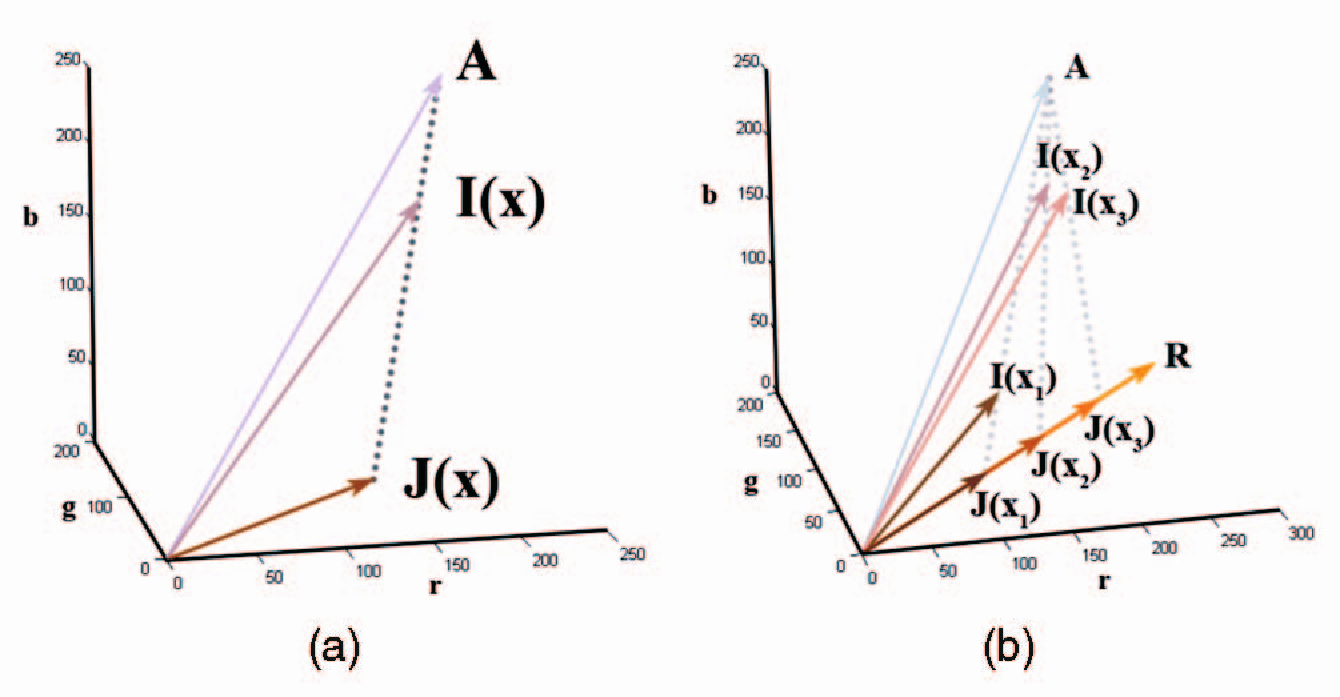
\includegraphics[width=0.8\textwidth]{./imgs/g711.png}
    \caption{传递函数}
    \label{fig-trans-dark}
 \end{figure}

去雾的传递函数与大气光以及暗通道的关系如公式\eqref{eq-trans-dark}所示,其在线性空间的表示可见于图\ref{fig-trans-dark}。

\begin{equation}
    t_r(x,y) = \frac{A_r^c - I^c(x,y)}{A_r^c - I_d^c(x,y)}
    \label{eq-trans-dark}
\end{equation}

根据图\ref{fig-dehazy}的流程,我们可以编写出该算法伪代码\ref{algo-DCP}。

\begin{algorithm}[t]
    \caption{DCP}
    \label{algo-DCP}
    \textbf{输入:} 有雾图像$I_h^c(x,y)$,滤波器核大小$W$,透视雾保留系数$\omega$,导向滤波器半径$r$,估计大气光使用的像素比例$p$
    \begin{algorithmic}
    \State 使用灰度化有雾图像$I_g^c(x,y)$计算有雾图像暗通道$I_d^c(x,y)$,根据暗通道 $I_d^c(x,y)$,获取最小$pMN\dim$个像素的位置
    \State 根据有雾图像中对应的位置的像素值估计每个通道的$A_r^c$
    \State 估计传递函数$\hat t_r(x,y) = 1 - \omega \min\limits_{c\in{r,g,b}}\frac    {I_h^c(x,y)}{A_r^c}$
    \State 对传递函数进行导向滤波$\hat t_r(x,y)$,获取最终传递函数$t_r(x,y)$
    \State 根据大气光$A_r^c$与传递函数$t_r(x,y)$估计去雾图像$\hat I^c(x,y) = \frac{I_h^c(x,y) - A_r^c}{t} + A_r^c$
    \State \Return 去雾图像$\hat I^c(x,y)$
    \end{algorithmic}
\end{algorithm}

\subsection{边界约束和上下文正则化的单图像去雾}
Meng等人\cite{meng.pan201312}提出了一种带有边界约束和上下文正则化的SID方法(BCL),对传输函数加上固有探索边界约束,再结合基于加权L1范数的上下文正则化,提高未知场景的传递函数估计质量,具体如图\ref{fig-trans-c}所示。加入闭运算、2dfft与圆形滤波器组来进一步减弱图像噪声,增强图像结构。

\begin{figure}[htbp]
    \centering
    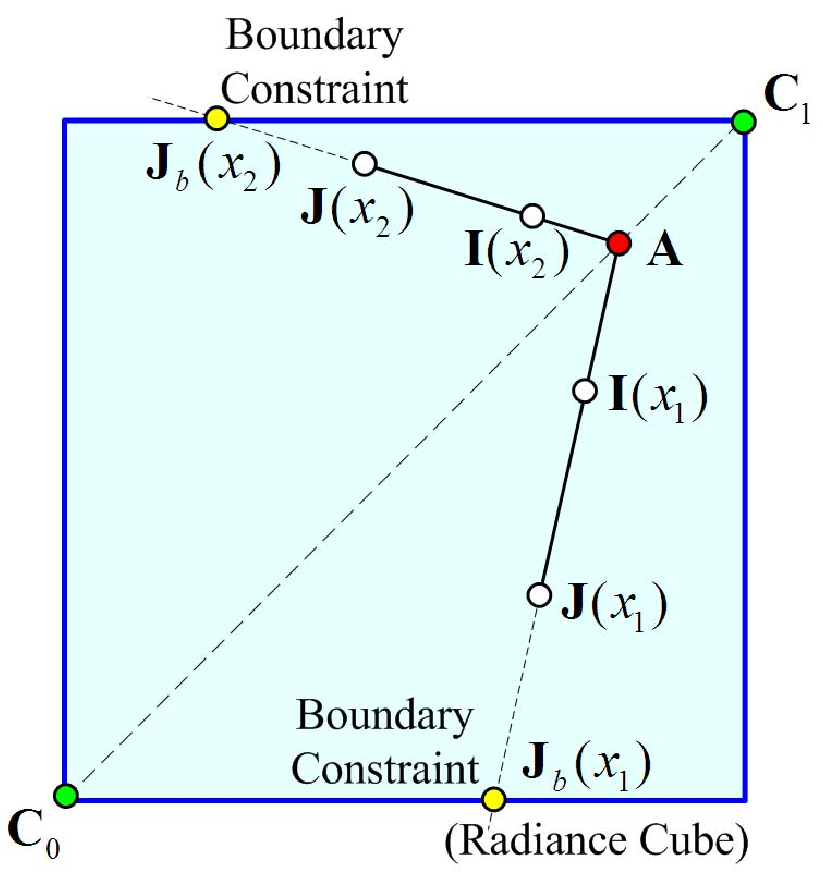
\includegraphics[width=0.8\textwidth]{./imgs/g712.png}
    \caption{约束传递函数(其中$J(x) = I_h^c(x,y)$)}
    \label{fig-trans-c}
 \end{figure}

\begin{equation}
    t_r^* = \text{IFFT-2D}\left(\frac{\frac{\lambda}{\beta}\text{FFT-2D}(\hat t_r) + \sum\limits_{j\in k}\overline{\text{FFT-2D}(D_j)}\text{FFT-2D}(u_j)}{\frac{\lambda}{\beta} + \sum\limits_{j\in k}\overline{\text{FFT-2D}(D_j)}\text{FFT-2D}(u_j)}\right)
    \label{eq-trans-c}
\end{equation}

\begin{equation}
    D_j = \text{circularFilter}(\text{FFT-2D}(t_r), k_j)\quad(j\in k)
    \label{eq-dj}
\end{equation}

\begin{equation}
    u_j = \max{(\lvert D_j\rvert - \frac{W_j}{\text{length}(k)\times\beta} ,0)}\times \text{sign}(D_j)\quad(j\in k)
    \label{eq-uj}
\end{equation}

\begin{equation}
    W_j = e^{\frac{\text{circularFilter}(I_h^c(x,y), filter_j)}{2\sigma^2}}\quad(j\in k)
    \label{eq-wj}
\end{equation}

修正$t_r$如公式\eqref{eq-trans-c}表示其中$\lambda$为正则化系数,$\beta$为权重因子$k$为不同的滤波器核。公式\eqref{eq-dj}\eqref{eq-uj}\eqref{eq-wj}为一些变量的计算式,$\sigma$为预设方差。

根据图\ref{fig-dehazy}的流程,我们可以编写出BCL算法伪代码\ref{algo-BCL}。

\begin{algorithm}[t]
    \caption{BCL}
    \label{algo-BCL}
    \textbf{输入:} 有雾图像$I_h^c(x,y)$,滤波器核大小$W$,大气光上下界$C_1,C_0$,传递函数矫正系数$\epsilon\neq1$
    \begin{algorithmic}
    \State 对有雾图像进行最小值滤波,获取$I_m^c(x,y)$,$I_h^c(x,y)$的最大值就是每个通道的$A_r^c$
    \State 估计传递函数$\hat t_r(x,y) = \max{(\frac{A_r^c - I_h^c(x,y)}{A_r^c - C_0},\frac{I_h^c(x,y)-A_r^c}{C_1 - A_r^c})}$,对传递函数做$3\times 3$的腐蚀
    \State 使用公式\eqref{eq-trans-c}对加约束与规范化获取$t_r(x,y)$,矫正最终传递函数$t_r(x,y) = t_r(x,y)^\epsilon$
    \State 根据大气光$A_r^c$与传递函数$t_r(x,y)$估计去雾图像$\hat I^c(x,y) = \frac{I_h^c(x,y) - A_r^c}{t} + A_r^c$
    \State \Return 去雾图像$\hat I^c(x,y)$
    \end{algorithmic}
\end{algorithm}

\subsection{彩色椭球先验}
彩色椭球先验(Color Ellipsoid Prior,CEP)是一种基于统计的的单图像去雾算法,在218年被Bui等人提出\cite{bui.kim201802}。它一种基于模型的双色去雾方法,该方法在统计上对图像信号随机性具有鲁棒性,在各种雾度范围内有效执行,不需要任何后期细化过程,并且不会产生任何明显可见的噪声或光环工件。他们将 RGB 空间中的像素向量簇拟合到由像素值的矩构造的统计颜色椭圆体,提高了算法稳健性。所提出的方法不是为先验向量选择像素,而是使用椭球几何计算先验向量。计算出的先验向量在椭球表面的向量中具有最小的颜色分量,以便在大多数像素不饱和的任何程度的雾度中最大化去雾像素的对比度。为了避免光晕伪影,他们将模糊过程嵌入到彩色椭圆体的构造中,而不是应用高度复杂的后处理。以上先验向量在线性空间可表示为图\ref{fig-cep}形式。

\begin{figure}[htbp]
    \centering
    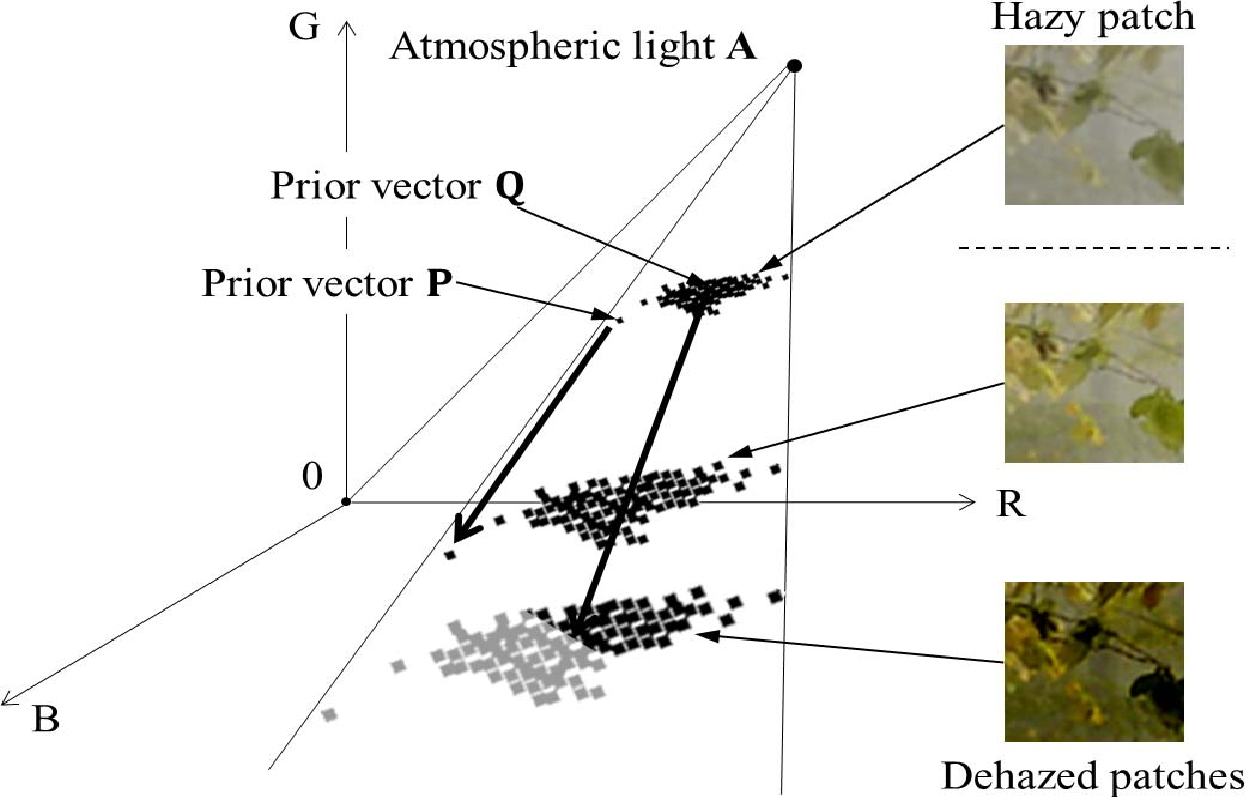
\includegraphics[width=0.8\textwidth]{./imgs/g713.png}
    \caption{椭球几何先验向量}
    \label{fig-cep}
 \end{figure}


 根据图\ref{fig-dehazy}的流程,我们可以编写出CEP算法伪代码\ref{algo-CEP}。

 \begin{algorithm}[t]
     \caption{CEP}
     \label{algo-CEP}
     \textbf{输入:} 有雾图像$I_h^c(x,y)$,滤波器核大小$W$,估计大气光使用的像素比例$p$,透视雾保留系数$\omega$
     \begin{algorithmic}
     \State 对有雾图像进行方框滤波,获取最小$pMN\dim$个像素的位置,根据有雾图像中对应的位置的像素值估计每个通道的$A_r^c$
     \State 使用导向滤波器/方形滤波器(快速)算椭圆向量,估计传递函数$\hat t_r(x,y)$
     \State 修正传递函数$t_r(x,y) = 1 - \omega\times \hat t_r(x,y)$
     \State 根据大气光$A_r^c$与传递函数$t_r(x,y)$估计去雾图像$\hat I^c(x,y) = \frac{I_h^c(x,y) - A_r^c}{t} + A_r^c$
     \State \Return 去雾图像$\hat I^c(x,y)$
     \end{algorithmic}
 \end{algorithm}
\subsection{非线性边界函数的传输下界}
Raikwar等人\cite{raikwar.tapaswi2020}在Meng等人\cite{meng.pan201312}基础上,提出了一种非线性的边界约束方法(记作NLB),通过理论计算出准确的传输函数的下界,进一步优化了算法。他们所提出的方法通过将传输估计问题转化为有雾图像和无雾图像之间的差异估计,来提高准确性。相比于BCL,NLB主要是修改了传输函数的估计(见公式\eqref{eq-tr-low}与\eqref{eq-delta}),次要变化为修改了以下滤波器组的核系数与假定了每个通道的环境光是一致的(见公式\eqref{eq-a})。

\begin{equation}
    \delta = \frac{1}{\min\limits_{c}I_h^c(x,y)} + \epsilon(x,y)
    \label{eq-delta}
\end{equation}

\begin{equation}
    A_r = \max{(A_r^r,A_r^g,A_r^b)}
    \label{eq-a}
\end{equation}

\begin{equation}
    t_r^{low}(x,y) = \frac{1}{1 + \frac{\max{(\min\limits_{c}I_h^c(x,y))}\times 10^{-0.05\zeta\delta}}{A_r - \min\limits_{c}I_h^c(x,y)}}
    \label{eq-tr-low}
\end{equation}

\begin{equation}
    \hat t_r(x,y) = \left\{\begin{matrix}t_r^{low}(x,y), & \text{if } A_r - \min\limits_{c}I_h^c(x,y) > 0.\\
        \frac{\lvert t_r^{low}(x,y) \rvert}{z}, & \text{otherwise}\\\end{matrix}\right. \qquad z = \max \lvert t_r^{low}(x,y) \rvert
    \label{eq-tr-nlb}
\end{equation}

根据图\ref{fig-dehazy}的流程,我们可以编写出NLB算法伪代码\ref{algo-NLB}。

\begin{algorithm}[ht]
    \caption{NLB}
    \label{algo-NLB}
    \textbf{输入:} 有雾图像$I_h^c(x,y)$,滤波器核大小$W$,传递函数矫正系数$\epsilon\neq1$,下界估计参数$\zeta$
    \begin{algorithmic}
    \State 对有雾图像进行最小值滤波,获取$I_m^c(x,y)$,$I_h^c(x,y)$的最大值就是每个通道的$A_r^c$
    \State 根据公式\eqref{eq-tr-low}估计传递函数下界$t_r^{low}(x,y)$,对传递函数做$3\times 3$的腐蚀
    \State 根据公式\eqref{eq-tr-nlb}估计传递函数$\hat t_r(x,y)$,对传递函数做$3\times 3$的腐蚀
    \State 使用公式\eqref{eq-trans-c}对加约束与规范化获取$t_r(x,y)$,矫正最终传递函数$t_r(x,y) = t_r(x,y)^\epsilon$
    \State 根据大气光$A_r^c$与传递函数$t_r(x,y)$估计去雾图像$\hat I^c(x,y) = \frac{I_h^c(x,y) - A_r^c}{t} + A_r^c$
    \State \Return 去雾图像$\hat I^c(x,y)$
    \end{algorithmic}
\end{algorithm}